% ===============================================================
% =							Work Plan	 						=
% ===============================================================
% # SECTION: Plano de Trabalho #
\chapter{Work Plan}
\label{cha:work_plan}

This chapter, presented the work done so far, as well as the work plan and necessary tasks to conclude the development of the proposed solution.

\section{Previous Work}
\label{sub:previous_work}

For a better understanding of the technologies that are going to be used, we conducted a few experiments integrating OpenCV with Android.
Already described in Section \ref{sub:eval_applications}, \citeauthor{datta2006studying} \cite{datta2006studying} implemented a system capable of extracting features of a photograph and give a classification based on a set of features extracted.
For the first experiment, we started by implementing three of those features in real-time. After receiving each frame captured by the phone's camera, we started by converting the frames from RGB to HSV color space. After converting, we obtained three 2-dimensional matrices corresponding to each of the HSV components. For each of the matrices, we calculated the average pixel intensity to characterize the use of light (V), the saturation average as the saturation indicator (S) and similarly for the hue (H). Currently, the interpretation of the values might not be clear. For HSV, Hue range is $[0,179]$, Saturation range is $[0,255]$ and Value range is $[0,255]$ \cite{OCV}.

The calculation of such features can be defined as:
\begin{equation}
Av_{k} = {{1 \over XY} {\sum_{x=0}^{X-1}{\sum_{y=0}^{Y-1}{I_{k}(x,y)}}}}
\label{eq:average_hsv}
\end{equation}

where $k$ can take the value $[h,s,v]$ which corresponds to each of the matrices obtained before. $X$ and $Y$ correspond to the dimension of the image, and $x$ and $y$ to the position of that pixel in the matrix.
The calculated averages are then presented to the user in the viewfinder (Figure \ref{fig:experiment1}).

\begin{figure}[htbp]
    \centering
    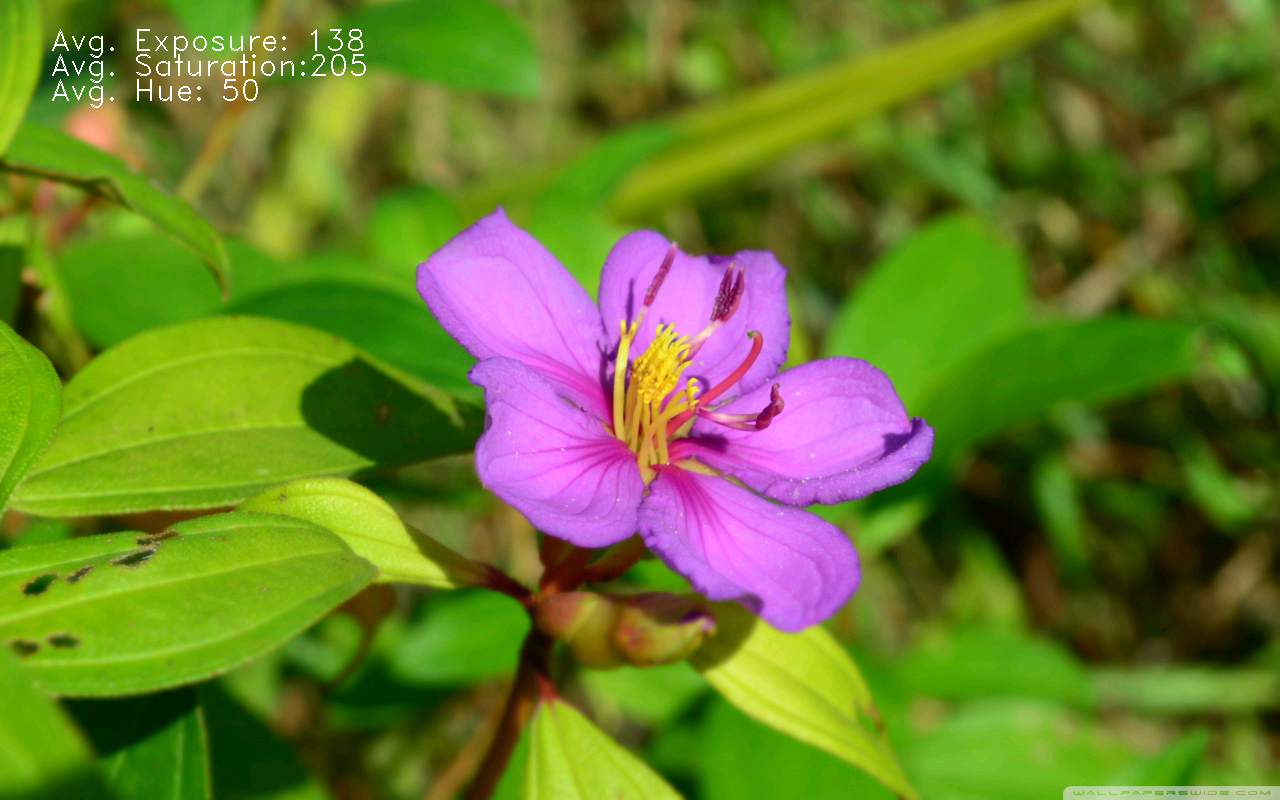
\includegraphics[scale=0.25]{experiment1.png}
	\caption{Experiment displaying average values of hue, saturation and value calculated with equation \ref{eq:average_hsv}\cite{datta2006studying}.}
	\label{fig:experiment1}
\end{figure}

As a second experiment we experimented a visualization of detecting a triangular composition (Section \ref{subsub:rule_triangles}). In every frame received from the camera, the device detects the first three faces and draws a triangle between them, serving as a visual cue for a better rearrangement of the subjects (Figure \ref{fig:experiment2}).

\begin{figure}[htbp]
    \centering
    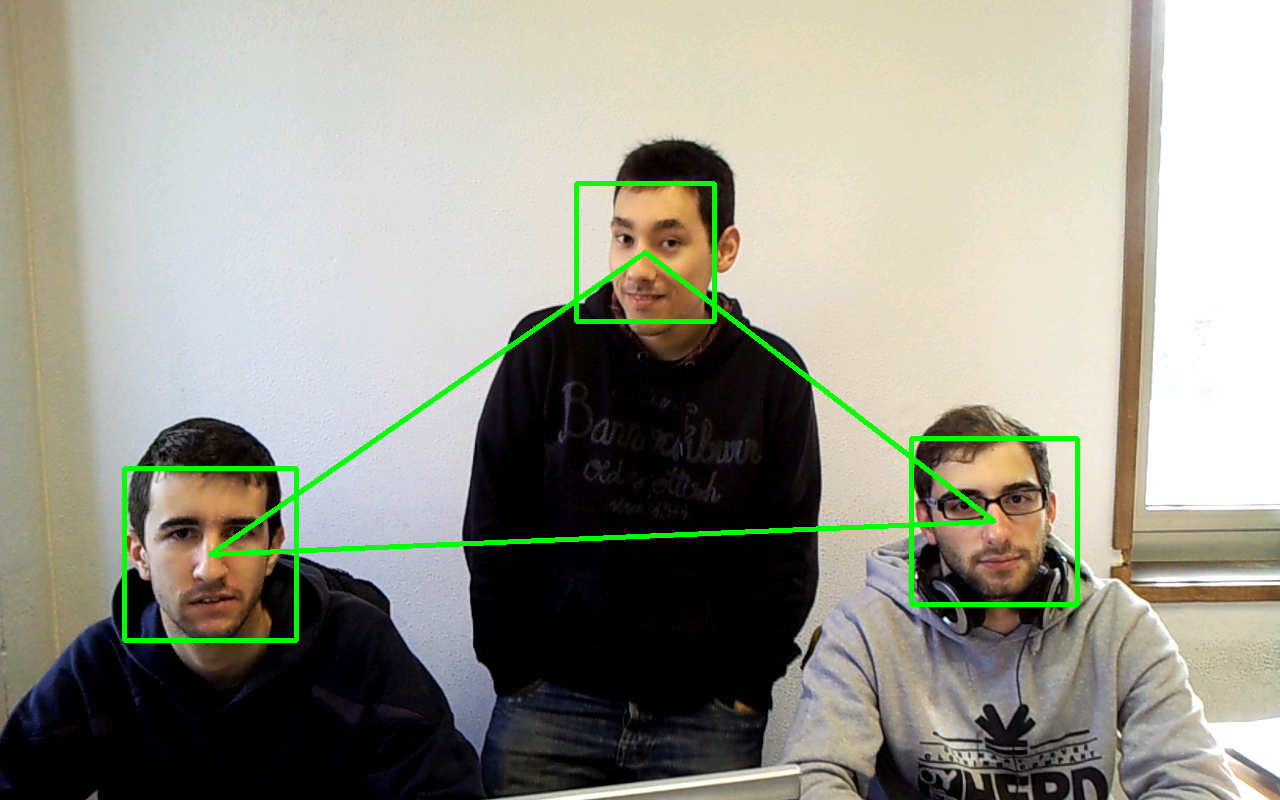
\includegraphics[scale=0.25]{experiment2.png}
	\caption{Experiment with triangle drawn with detected faces.}
	\label{fig:experiment2}
\end{figure}

This experiment was made using a Cascade Classifier in JAVA and C++ implemented by OpenCV. Both Cascade Classifiers used the same pre-trained classifier for frontal face detection. JAVA's classifier presented a better performance in both speed and detection. C++'s classifier was unable to detect faces between consecutive frames with minimum or without movement.

\section{Work Plan}
\label{sub:work_plan}

To develop the proposed solution a work plan is presented with a set of tasks to accomplish over time, as well as some that have been completed or are in progress. Divided into six major tasks, Figure \ref{fig:workplan_diagram} contains a detailed schedule of tasks to be performed and respective duration.

The first group is dedicated to the final document to be delivered, that will include the state of the art study and all of the developed work. The document will be written in parallel with the other tasks.

The second group involves the study of the state of the art. It involves a study of related applications for image capture and process, and a study of rules of composition that can be applied in the scenario that our approach covers. Some applications are already described in Section \ref{sub:capturing_processing} and Section \ref{sub:previous_work} describes experiments already made.

The group entitled Related Work, involves tasks that lead to a better understanding of the subject of this thesis and state of the art. Ideas and necessary techniques to develop our proposed solution, are also included in this group.

How this application will interact with the user, is something that should be taken in consideration. The fourth group, consists of tasks related to the mobile interface design and how it will react the user input.

The Development group consists of tasks related to the development of the application. It is divided in two subtasks that include the development of the interface previously designed, the responses from received inputs and the functionalities available. As mentioned before, these functionalities must allow a user to capture images and edit them. To support the main subject of this dissertation, functionalities related to the evaluation of a scene are also included. The mobile application will be developed in Android and C++ using the OpenCV \cite{OCV} framework. 

The final application will be put to a series of system and usability tests. Two groups of people will be used for usability evaluation, by testing how they react to the interface and how they expect it to react. One of the groups will contain people with enough knowledge in photography to be considered as an amateur or professional photographer. The remaining group will be composed of people that don’t have any knowledge in the area.
\begin{figure}[htbp]
    \centering
    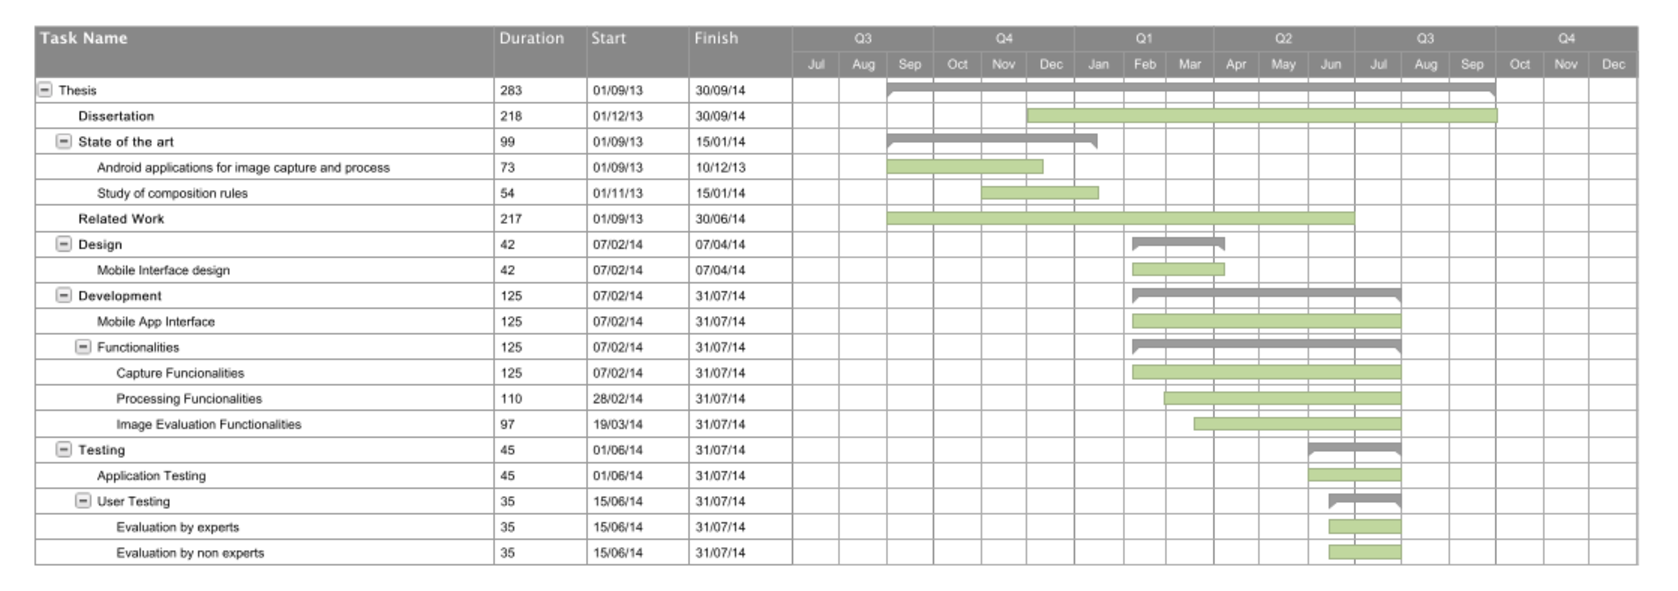
\includegraphics[width=0.98\textheight,angle=90]{workplan.pdf}
	\caption{Task schedule represented by a Gantt diagram.}
	\label{fig:workplan_diagram}
\end{figure}